
\newrefcontext[sorting=ynt]

\lettrine{I}{ntraspecific} competition is an important driver of population dynamics and the spatial distribution of organisms \citep{krebs1978}, and has two main types, `exploitation' and `interference'.
In exploitation competition, individuals compete indirectly by depleting a common resource, while in interference competition, individuals compete directly by interacting with each other \citep{birch1957,case1974,keddy2001}.
A special case of interference competition which is widespread among animal taxa is `kleptoparasitism', in which an individual steals a resource from its owner \citep{iyengar2008}.
Since competition has an obvious spatial context, animals should account for the locations of competitors when deciding where to move \citep{nathan2008a}.
This is expected to have downstream effects on animal distributions across spatial scales, from resource patches \citep{fretwell1970}, to species distributions \citep{duckworth2007,schlagel2020}.
Animal movement strategies are thus likely to be adaptive responses to landscapes of competition, with competitive strategies themselves being evolved responses to animal distributions.
Empirical studies of this joint evolution are nearly impossible at large spatio-temporal scales.
This makes models linking individual movement and competition strategies with population distributions necessary.

Contemporary individual-to-population models of animal space-use \citep[reviewed in][]{deangelis2019} and competition, however, are only sufficient to represent very simple movement and prey-choice decisions.
\graffito{
    These classical foraging models correspond to real conditions as much as macro-economic models do with the real world.
    They are likely useful only at very broad scales.
}
For example, models including the ideal free distribution \citep[IFD;][]{fretwell1970}, information-sharing models \citep[][]{giraldeau1999,folmer2012}, and producer-scrounger models \citep[][]{barnard1981,vickery1991,beauchamp2008}, often treat foraging competition in highly simplified ways.
Most IFD models consider resource depletion unimportant or negligible \citep[continuous input models, see][]{tregenza1995, vandermeer1997}, make simplifying assumptions about interference competition, or even model an \textit{ad hoc} benefit of grouping \citep[e.g.][]{amano2006b}.
Meanwhile, producer-scrounger models primarily examine the benefits of choosing either a producer or scrounger strategy given local conditions, such as conspecific density \citep{vickery1991}, or the order of arrival on a patch \citep{beauchamp2008}.
Overall, these models simplify the mechanisms by which competition decisions are made, and downplay spatial structure \citep[see also][]{holmgren1995, garay2020, spencer2018}.

On the contrary, spatial structure is key to foraging (competition) decisions \citep{beauchamp2008}.
How animals are assumed to integrate the costs (and potential benefits) of competition into their movement decisions has important consequences for theoretical expectations of population distributions \citep{vandermeer1997,hamilton2002,beauchamp2008}.
In addition to short-term, ecological effects, competition also likely has evolutionary consequences for individual \textit{movement strategies}, setting up feedback loops between ecology and evolution.
Modelling competition and movement decisions jointly is thus a major challenge.
Some models take an entirely ecological view, assuming that individuals move or compete ideally, or according to fixed strategies \citep{vickery1991,holmgren1995,tregenza1995,amano2006b}, but see \citep{hamilton2002}.
Models that include evolutionary dynamics in movement \citep{dejager2011,dejager2020} and foraging competition strategies \citep{beauchamp2008,tania2012} are more plausible, but they too make arbitrary assumptions about the functional importance of environmental cues to individual decisions.

Mechanistic, individual-based models are well suited to capturing the complexities of spatial structure, animal decision-making, and evolutionary dynamics \citep{guttal2010,kuijper2012,getz2015,getz2016,white2018,long2020,netz2021a}; for conceptual underpinnings see \textcite{huston1988,mueller2011,deangelis2019}.
\graffito{
    I've been lucky enough to have been taught by, or to have met, many of these authors, including Vishu Guttal, Iain Couzin, Wayne Getz, Thomas M\"uller, and Don DeAngelis.
}
% \graffito{
%     Reading Lauren White's implementation of movement decisions as resource selection functions \citep{white2018} was instrumental in how I thought about my work.
%     Her model also inspired Chapter~\ref{ch:pathomove}.
% }
Individual-based models can incorporate the often significant variation in movement and competition preferences found in populations, allowing individuals to make different decisions given similar cues \citep[][]{laskowski2013}.
Individual-based models also force researchers to be explicit about their modelling assumptions, such as \textit{how exactly} competition affects fitness.
Similarly, rather than taking a purely ecological approach and assuming individual differences \citep[e.g. in movement rules:][]{white2018}, allowing movement strategies to evolve in a competitive landscape can reveal whether individual variation emerges in plausible ecological scenarios \citep[as in][]{getz2015}.
This allows the functional importance of environmental cues for movement \citep[see e.g.][]{scherer2020} and competition decisions in evolutionary models to be joint outcomes of selection, and lets different competition strategies to be associated with different movement strategies \citep[][]{getz2015}.

Here, we present a spatially-explicit, mechanistic, individual-based model of intraspecific foraging competition, where movement and competition strategies jointly evolve on a resource landscape with discrete, depletable food items that need to be processed (`handled') before consumption.
\graffito{
    The Kleptomove model's source code is adapted from an earlier predator-prey model
    \citep{netz2021a}.
}
In our model, foragers make movement decisions using inherited, evolvable preferences for local ecological cues, such as resource and competitor densities; the combination of preferences for each cue forms individuals' movement strategy \citep[similar to relative step-selection:][]{fortin2005, avgar2016}.
Lifetime resource consumption is our proxy for fitness; more successful individuals produce more offspring, transmitting their movement and foraging strategies to future generations (with small mutations).
We consider three scenarios: in the first scenario, we examine only exploitation competition.
In the second scenario, we introduce kleptoparasitic interference as an inherited strategy, fixed through an individual's life.
In the third scenario, we model kleptoparasitism as a behavioural strategy conditioned on local environmental and social cues; the mechanism underlying this foraging choice is also inherited.

Our model allows us to examine the evolution of individual movement strategies, population-level resource intake, and the spatial structure of the resource landscape.
The model enables us to take ecological snapshots of consumer-resource dynamics (animal distributions, resource depletion, and competition) proceeding at evolutionary time-scales.
Studying these snapshots allows us to check whether, when, and to what extent the spatial distribution of competitors resulting from the co-evolution of competition and movement strategies corresponds to standard IFD predictions.
We investigate \textit{(1)} which movement strategies evolve in our three competition scenarios, \textit{(2)} whether movement strategies differ within and between competition strategies in our scenarios, and \textit{(3)} whether the emergent spatial distributions of consumers corresponds to `ideal free' expectations.

\section*{The Model}

Individual-based models have to explicitly specify numerous assumptions (e.g. spatial structure, individual interactions, event timescales), but this helps expose assumptions that are often hidden below the surface in analytical models. 
We kept our model assumptions as simple and generic as possible, striving for general, conceptual insights.
To keep the model realistic, we based it on the foraging behavior of shorebirds such as oystercatchers (\textit{Haematopus} spp.), which are extensively studied in the context of foraging competition, both empirically \citep[e.g.][]{vahl2005, vahl2005a,vahl2007, rutten2010, rutten2010a}, and using individual-based models \citep[reviewed in][]{stillman2010}.

\graffito{
    We initially tried 100 timesteps, but settled on 400 as this allowed enough time for individuals' intake to be a function of their movement strategy, rather than their good fortune in being initialised in a productive part of the landscape.
}
Our environment is a fine grid of cells, and each grid cell can hold multiple individuals.
Resources are discrete, as is our conception of time within and between generations. 
Our population, with a fixed number of individuals (N = 10,000), moves on a landscape of 512\textsuperscript{2} grid cells (approx. 1 individual per 26 cells), with wrapped boundaries (i.e., a torus); individuals passing beyond the bounds at one end re-appear on the opposite side.
The model has two time scales, first, an ecological time scale of $T$ timesteps comprising one generation (default $T$ = 400), during which individuals move, make foraging decisions, and handle prey-items they find or steal.
Individuals are immobile while handling food items, creating the conditions for kleptoparasitism \citep{brockmann1979,ruxton1992}.
At the end of each generation, individuals reproduce, transmitting their movement and foraging strategies to their offspring, whose number is proportional to individual intake at the ecological time scale.
Our model has 1,000 generations, and this comprises the evolutionary timescale.

\subsection*{Resource Landscape}

\paragraph{Prey Abundance}

\graffito{
    Early versions of this model had one giant resource peak; this was dropped as it was relatively easy for individuals to find their way to productive areas.
}
We considered our discrete resources, called `prey-items' to represent mussels, a common prey of many shorebirds, whose abundances are largely driven by external gradients.
We assigned each cell a constant probability of generating a new prey-item per timestep, which we refer to as the cell-specific growth rate $r$.
We modelled clustering in landscape productivity by having the distribution of $r$ across the grid take the form of 1,024 resource peaks, placed at regular distances of 16 grid cells from the peaks around them; $r$ declines from the centre of each peak (called $r_{max}$) to its periphery (see Fig.~\ref{klepto_fig_01}A).
Thus the central cell generates prey-items five times more frequently than peripheral cell: at $r_{max}$ = 0.01, central cells generate one item per 100 timesteps (four items/generation), while the peripheral cells generate one item only every 500 timesteps ($<$ one item/generation).
All landscape cells have a uniform carrying capacity $K$ of 5 prey-items.
While a cell is at carrying capacity its $r$ is 0.
Cells are initialised with prey-items proportional to their $r$ (see e.g. Fig.~\ref{klepto_fig_01}A).

\paragraph{Prey Acquisition by Foragers}

Foragers perceive a cue indicating the number of prey-items $P$ in a cell, but fail to detect each item with a probability $q$, and are thus successful in finding a prey-item with a probability $1 - q^P$.
Individuals on a cell forage in a randomised sequence, and the probability of finding a prey-item ($1 - q^P$) is updated as individuals find prey, reducing $P$.
Foragers that find a prey-item must handle it for a fixed handling time $T_H$ (default = 5 timesteps), before consuming it \citep[][]{ruxton1992}.
Natural examples include the time required for an oystercatcher to break through a mussel shell, or a raptor to subdue prey; overall, the handling action is obvious, and the prey is not fully under the control of the finder \citep{brockmann1979}.
Foragers that do not find a prey-item are considered idle in that timestep, and are counted as `non-handlers'.
Similarly, handlers that finish processing their prey in timestep $t$ can only forage again in timestep $t+1$, i.e., they are idle in the timestep $t$.

\subsection*{Movement Strategies}

All individuals move simultaneously at the end of each timestep $t$, and then implement their foraging or kleptoparasitic behaviour to acquire prey.
However, handlers do not make any movements until they have fully handled and consumed their prey.
We model movement as comprised of small, discrete steps between adjacent cells.
Across scenarios, individuals make movement decisions using evolved cue preferences.
Individuals select a destination cell, after assessing potential destinations based on available cues, similar to approaches used previously \citep{getz2015,getz2016,white2018,scherer2020,netz2021a}.

\graffito{
    Our individuals can use much more complex functions, encoded by neural networks, an idea that has been explored, but not widely used, in movement ecology \citep{mueller2011}.
}
To move, individuals scan the nine cells of their Moore neighbourhood for three environmental cues, \textit{(1)} an indication of the number of discrete prey-items $P$, \textit{(2)} the number of individuals handling prey $H$ (`handlers'), and \textit{(3)} the number of individuals not handling prey $N$ (`non-handlers').
Individuals rank the potential destinations (including their current cell) by their suitability $S$, where $S = s_PP + s_HH + s_NN$, and move to the most suitable cell in timestep $t+1$.
The individual preferences for each cue, $s_P$, $s_H$, and $s_N$, have numeric values, are considered to be evolvable traits that can be transmitted between generations, and undergo independent mutation.
Since individuals are constrained to perceiving and moving short distances, they may not always sense their best long-term move.

It is the combination of cue preferences, and especially their value relative to each other, that determines individual movement decisions \citep[similar to relative selection coefficients,][]{fortin2005,avgar2016,white2018}. 
For example, an extreme value of $s_P$ relative to the other preferences would mean that an individual's movement decisions are guided primarily by differences in the local density of prey-items.
We call an individual's combination of inherited preferences its \textit{movement strategy} (see e.g. Fig.~\ref{klepto_fig_01}E).

\subsection*{Competition Strategies}

\paragraph{Scenario 1: Exploitative Competition}

In scenario 1, we simulate only exploitative competition; individuals (henceforth called `foragers') move about on the landscape and probabilistically find, handle, and consume prey-items.
Foragers can be either in a `searching' or a `handling' state \citep{holmgren1995}.

\paragraph{Scenario 2: Foraging or Kleptoparasitism as Fixed Strategies}

\graffito{
    The Kleptomove simulation can be modified to change the probability of kleptoparasite success.
}
In scenario 2, the competition strategy is genetically determined and transmitted from parents to offspring: exploitative competition (by foragers), or kleptoparasitic interference (by kleptoparasites).
Kleptoparasites cannot extract prey-items directly from the landscape, and only steal from handlers \citep[see][]{holmgren1995}.
Kleptoparasites are always successful in stealing from handlers, and such successful surprise attacks are commonly observed among birds \citep{brockmann1979}.
When multiple kleptoparasites target the same handler, only one (randomly selected) is considered successful --- thus kleptoparasites compete exploitatively among themselves.
Kleptoparasites displace the handler that they robbed of prey up to 5 cells away from their location.
Having acquired prey, kleptoparasites become handlers, but need only handle prey for $T_H - t_h$ timesteps, where $t_h$ is the time that the prey has already been handled by its previous owner.
Once a kleptoparasite becomes a handler, it can also be targeted by other kleptoparasites.
Unsuccessful kleptoparasites are considered idle, and are counted as non-handlers.
Movement strategies evolve independently of the competition strategy, as in scenario 1; however, the optimal movement strategy for foragers need not be the same as that for kleptoparasites.

\paragraph{Scenario 3: Conditional Interference Competition}

\graffito{
    Similar to movement decisions, competition decisions can also be encoded by a neural network.
}
In scenario 3, each individual can either act as a forager, or as a kleptoparasite, depending on its assessment of local conditions.
Similar to how movement decisions are made based on local cues, individuals process cell-specific environmental cues in timestep $t$ to determine their competition strategy in the next timestep as
% \begin{linenomath*}
\begin{equation}
    \text{strategy} = 
\begin{cases}
    \text{forager},& \text{if } w_PP + w_HH + w_NN \geq w_0\\
    \text{kleptoparasite},              & \text{otherwise}
\end{cases}
\end{equation}  
% \end{linenomath*}
where the cue preferences $w_P$, $w_H$ and $w_N$, and the threshold value $w_0$, are numeric values, and heritable between generations (with small, rare, independent mutations).
The combination of the cue preferences for competition decisions forms each individual's \textit{competition strategy}.
Individuals' competition strategies may lead to specialisation as foragers or kleptoparasites (as in scenario 2), or to plastic behaviour conditioned on local cues.
The competition dynamics are the same as in scenario 2.

\subsection*{Reproduction and Inheritance}

Our model considers a population of fixed size (10,000 individuals) with discrete, non-overlapping generations. 
For simplicity, we assume that individuals are haploid and reproduction is asexual. 
In scenarios 1 and 2, individuals only inherit and transmit their cue preferences ($s_P$, $s_H$, $s_N$) which determine movement decisions.
In scenario 3, individuals also inherit cue preferences for competition decisions ($w_P$, $w_H$, $w_N$, $w_0$), and transmit them to offspring.
The movement and competition cue preferences all mutate independently in scenario 3.
\graffito{
    The implicit assumption here is fecundity effects, rather than mortality effects. This is consistent with many shorebirds, which often fail to breed in bad years, but have very high adult survival.
}
Each individual's number of offspring is proportional to the individual's total lifetime intake of resources; hence, resource intake is used as a proxy for fitness. 
A weighted lottery (with weights proportional to lifetime resource intake) selects a parent for each offspring in the subsequent generation \citep[see e.g.][]{tania2012,netz2021a}.
Across scenarios, the cue preferences for movement decisions are subject to rare, independent mutations ($\mu$ = 0.001).
The mutational step size (either positive or negative) is drawn from a Cauchy distribution with a scale of 0.01 centred on zero, allowing for a small number of very large mutations while most mutations are small.
In scenario 2, foragers may infrequently mutate into a kleptoparasite (or \textit{vice versa}; $\mu$ = 0.001).
In scenario 3, the competition cue preferences also mutate as described above.
Each offspring is initialised at random locations on the landscape, leading individuals to experience conditions potentially different from those of their parent.
We chose this option because it allows us to focus on adaptive movement strategies, whereas limited dispersal confounds movement and local adaptation.

\subsection*{Simulation Output and Analysis}

\graffito{
    The simulation output, in a Windows-specific compressed format, required a number of specialised functions to extract useful information.
}
We ran all three scenarios at a default $r_{max}$ of 0.01, which we present in the \textsc{Results}, and also across a range of $r_{max}$ values between 0.001 and 0.05 (see Fig.~\ref{klepto_fig_06} and Supplementary Material Figs. 7 -- 9).
We initialised the cue preferences with values drawn from a Cauchy distribution with a scale of 0.01 centred on zero; this allows a very small amount of variation in the population (see e.g. Fig.~\ref{klepto_fig_01}E), and is equivalent to a single generation of mutation from all preferences initialised at zero (see \textsc{Reproduction and Inheritance} above).
Normalising each individual's cue preferences by the sum of the absolute values of all preferences $s_I = s_I / (|s_P| + |s_H| + |s_N|)$, for $s_I \in s_P, s_H, s_N$, makes it possible to visualise individuals on a three-dimensional trait space of relative preferences bounded by (-1.0: \textit{strongly avoid}, +1.0: \textit{strongly prefer}).
With remarkably consistent outcomes across replicates in each scenario, and as each simulation run produced massive datasets, we show the outcomes of three replicates here.
More data can be generated and analysed using the code linked below.

\paragraph{Population Activities and Intake}

Across scenarios, in each generation, we counted the number of times foragers were searching for prey, kleptoparasites were searching for handlers, and the number of timesteps that individuals of either strategy were handling a prey-item.
We refer to the ratio of these values as the population's `activity budget'.
We examined how the population activity budget developed over evolutionary time, and whether a stable equilibrium was reached.
Furthermore, we counted the population's mean per-capita intake per generation as a measure of population productivity.

\paragraph{Visualising Movement Strategies}

To understand the evolution of individual movement and competition strategies, we exported the cue preferences of each individual in every generation of the simulation.
We scaled each cue preference by the sum of the absolute values of the preferences, allowing us to plot individuals in a standardised three-dimensional trait space of relative cue preferences (with colour as an axis on a two-dimensional plot).
Individuals' position in this space allowed us to easily visualise and compare variation in movement strategies within and between competition strategies and across scenarios.

\paragraph{Visualising Scenario 3 Competition Strategies}

Scenario 3 competition strategies are determined by four values (3 preferences and threshold value), and competition decisions are outcomes of the interactions of these preferences with individuals' movement decisions and ecological conditions.
This makes strategies \textit{per se} difficult to visualise.
We first scaled the competition cue preferences and the threshold value as we did the movement cue preferences.
To illustrate variation in the competition strategies evolved, we presented each individual in representative generations (G = 10, 30, 100, 300, 950) with combinations of two key cues, handler and prey density (each 0 -- 5; 36 combinations overall).
We summarised the proportion of individuals that would attempt to steal at each combination of cue values (see Eqn. 1; Fig.~\ref{klepto_fig_04}F).

\paragraph{Ecological Snapshots of Consumer-Resource Distributions}

We exported snapshots of the entire simulation landscape at the mid-point of each generation ($t$ = 200).
Each snapshot contained data on \textit{(1)} the number of prey-items, \textit{(2)} the number of handling individuals, and the number of individuals using either a \textit{(3)} searching forager strategy or \textit{(4)} kleptoparasitic strategy, on each cell.
We used a subset of the total landscape (60\textsuperscript{2} of 512\textsuperscript{2} cells) for further analyses to speed up computation.
We determined the availability of direct resource cues for movement in each cell by calculating the cell-specific item gradient for each landscape snapshot, as the difference in prey counts between each cell and its neighbouring cells.
For each generation, we calculated the proportion of cells from which it was possible to sense differences in prey-items, i.e., a neighbouring cell with either more or fewer items.

\paragraph{Testing the Input Matching Rule}

A basic prediction of the IFD and the related matching rule is that the number of individuals on occupied patches should be proportional to patch productivity \citep{fretwell1970,parker1978,houston2008}.
Patch productivity is challenging to measure in real world systems, but is among our model's building blocks, and we examined the correlation between the number of individuals (excluding handlers) and the cell-specific productivity $r$, expecting large positive values.

\section*{Results}

\subsection*{Scenario 1: No Kleptoparasitism}

In scenario 1, foragers deplete prey-items faster than they are replenished, drastically reducing the overall number of prey within 50 generations (Fig.~\ref{klepto_fig_01}A).
The population activity budget is split between searching and handling (Fig.~\ref{klepto_fig_01}B); while handling and the mean per-capita intake are both initially low, they peak within ten generations (Fig.~\ref{klepto_fig_01}C), as individuals easily acquire prey-items from the fully stocked landscape in the first few generations.
With dwindling prey-items, fewer searching foragers find prey, and handling as a share of the activity budget declines to a stable $\sim$ 45\% within 50 generations, and mean per-capita intake also stabilises (Fig.~\ref{klepto_fig_01}C).
Across generations, the correlation between the number of foragers and cell productivity is only slightly positive (Fig.~\ref{klepto_fig_01}D).
This is in contrast with the perfect correspondence between resource input rate and forager density (the `input matching rule'), which is a defining property of the IFD \citep{parker1978, houston2008}.
Contrary to standard IFD assumptions, foragers cannot directly sense the local cell productivity $r$; instead they can only use the (small) number of prey-items available in a cell as a cue for local productivity.
A wide range of movement strategies co-exist on the landscape (see all generations in Supplementary Material Fig.~2, 6).
Some individuals mostly move up gradients of prey-items (Fig.~\ref{klepto_fig_01}E; $s_P$ $\approx$ 1.0), some move primarily towards successful foragers (handlers), while others move away from unsuccessful foragers which are potential competitors (more red $s_N$).

\begin{figure}[t!]
    \centering
    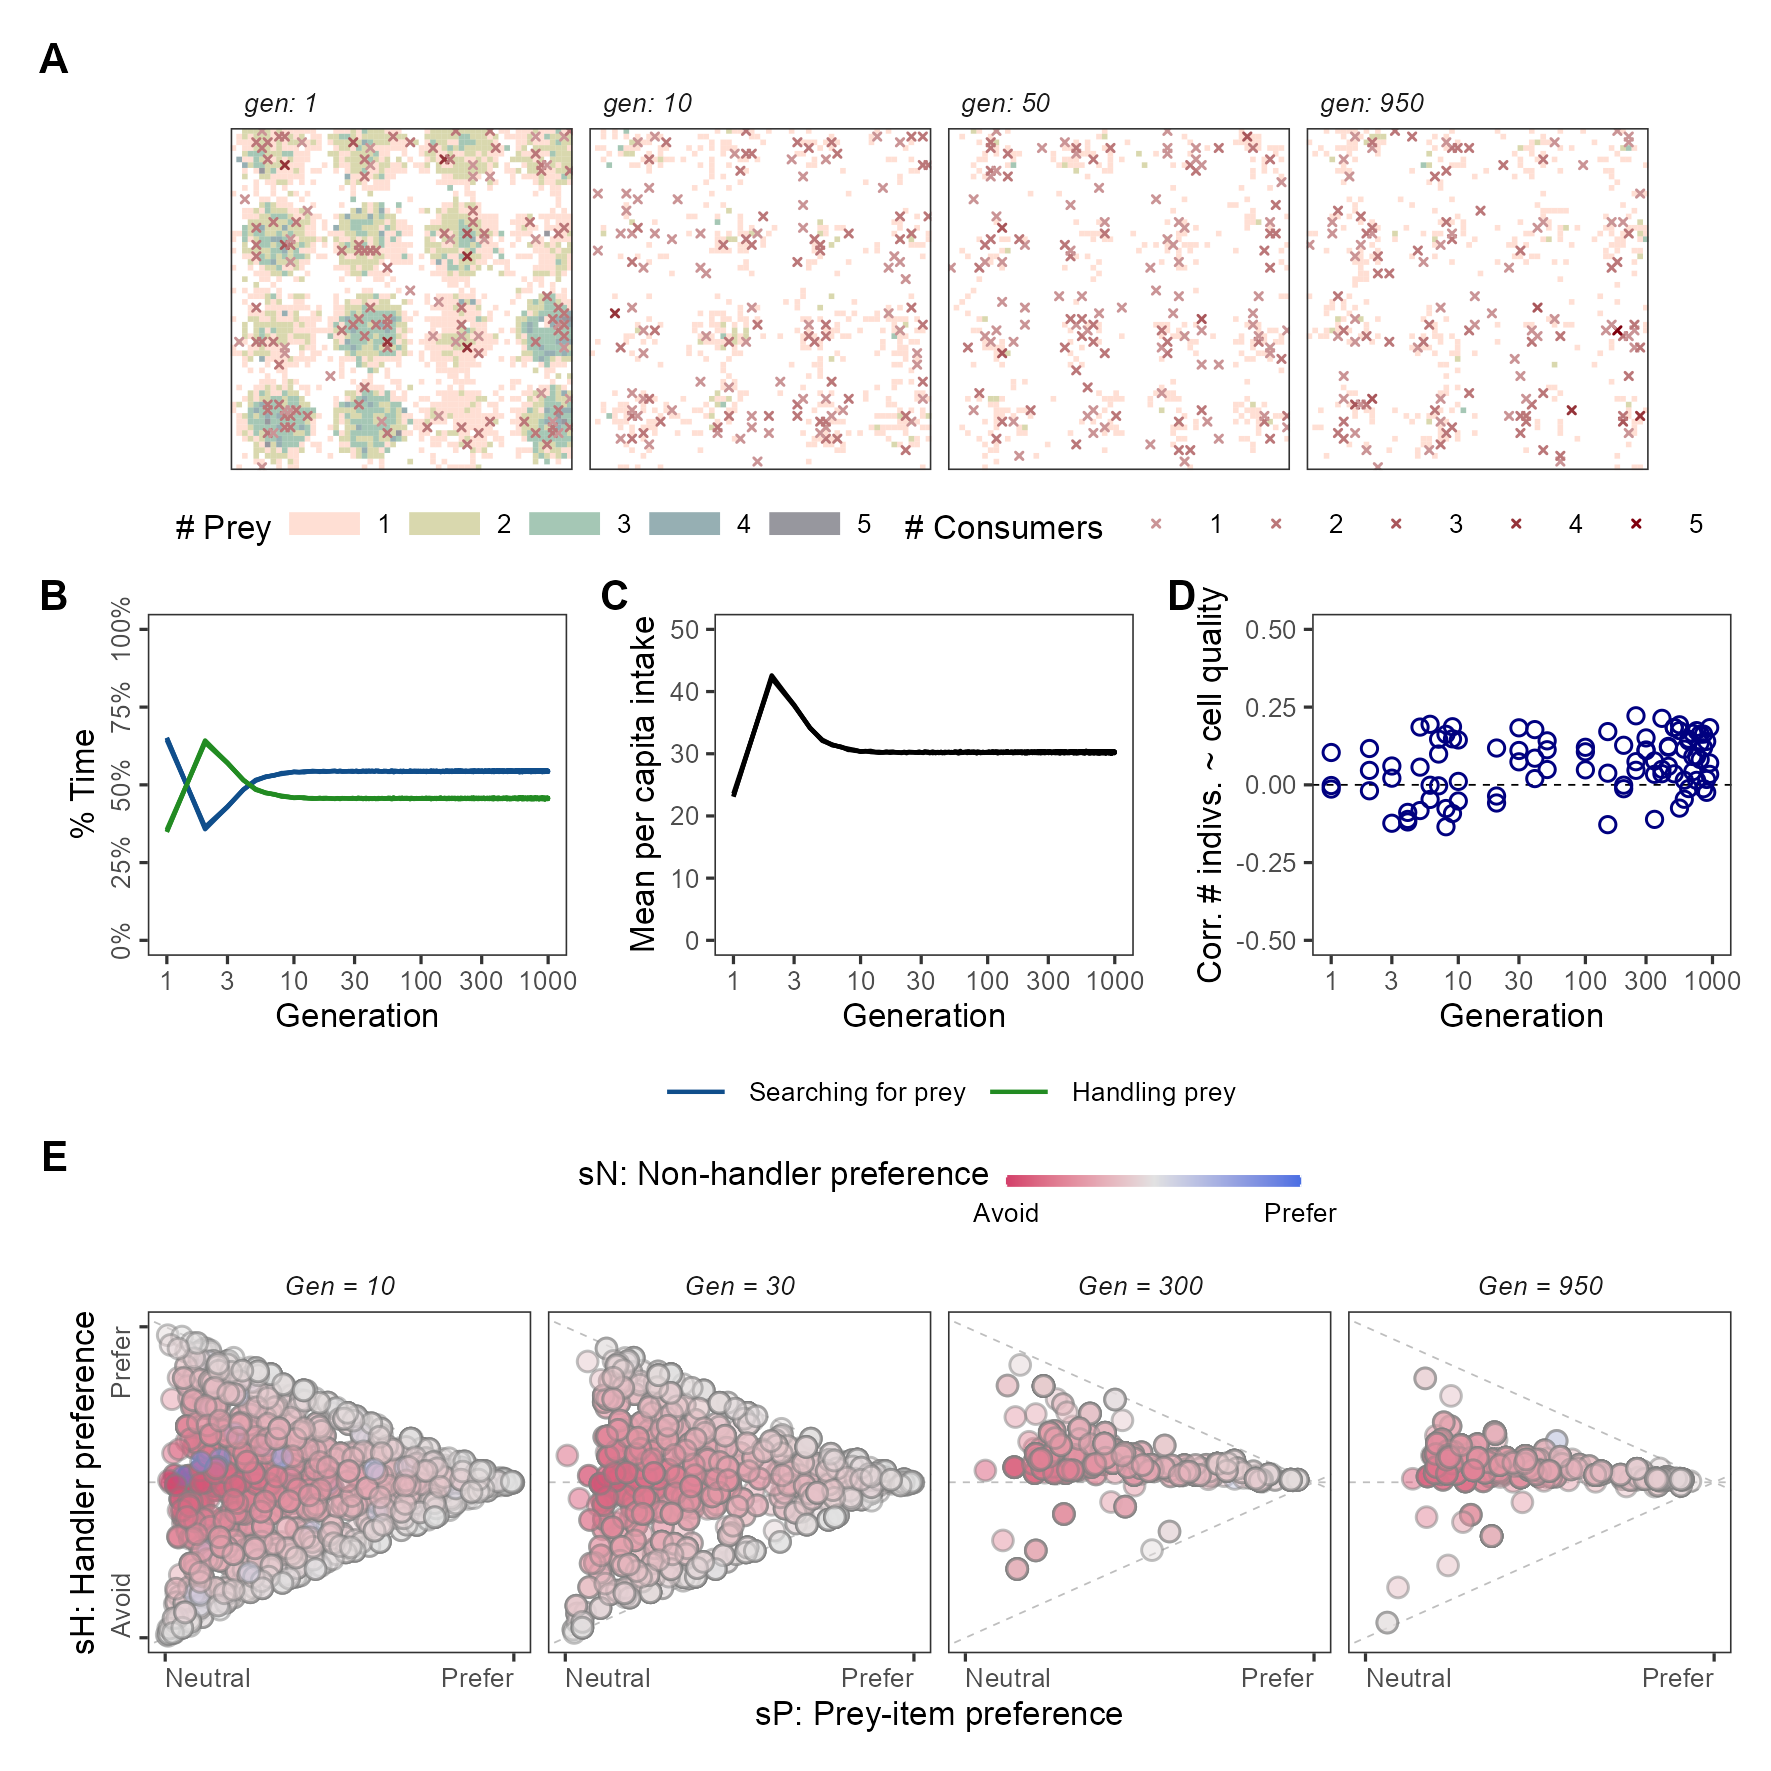
\includegraphics[width=0.9\textwidth]{figures/kleptomove/fig_01.png}
    \caption{
        \textbf{Eco-evolutionary implications of pure exploitation competition in scenario 1.}
        \textbf{(A)} A population comprised solely of foragers seeking prey on a resource landscape swiftly depletes initially abundant prey-items within 10 generations (of 1,000 simulated).
        Foragers maintain this prey-item scarcity throughout the remaining generations of the simulation, despite regular resource regeneration (see G = 950).
        \textbf{(B)} Within 20 generations of evolution, the population reaches an equilibrium in the relative proportion of time spent on searching for prey and handling prey, and in \textbf{(C)} mean per-capita intake.
        \textbf{(D)} The number of foragers per cell is only weakly correlated with cell productivity $r$, contrary to the input matching rule of Ideal Free Distribution theory.
        \textbf{(E)} A wide range of movement strategies co-exist on the landscape over hundreds of generations.
        Individuals may focus on moving up gradients of prey-items (sP $\approx$ 1.0: \textit{prefer}), moving towards successful foragers (handlers), or moving away from unsuccessful foragers which are potential competitors (sN $\approx$ red).
        Panels \textbf{A, E} show a single replicate, panels \textbf{B, C, D} and \textbf{D} show three replicate simulations with log-scaled X-axes (lines overlap almost perfectly); all panels are for $r_{max}$ = 0.01; panel \textbf{E} shows 2,500 individuals.
    }
    \label{klepto_fig_01}
\end{figure}

\subsection*{Scenario 2: Co-existence of Foragers and Kleptoparasites}

In scenario 2, with fixed foraging and kleptoparasitism allowed, the spatial distribution of prey-items at equilibrium is very different from scenario 1.
Consumers graze down resource peaks until few prey-items remain on the landscape; however, within 50 generations the resource landscape recovers with prey abundances higher than in the earliest generations (Fig.~\ref{klepto_fig_02}A).
This is because of the emergence of kleptoparasites (Fig.~\ref{klepto_fig_02}B): in early generations, kleptoparasites are rare, and the activity budget, the mean per-capita intake, and the distribution of consumers over the landscape, are similar to scenario 1.
As resources are depleted and kleptoparasite-handler encounters become more common than forager-prey encounters, kleptoparasitism becomes the majority strategy (a stable $\sim$70\% of the population; see Fig.~\ref{klepto_fig_02}B), and searching for handlers to rob becomes the commonest activity.
However, the high frequency of this activity and the low frequency of handling, indicate that few kleptoparasites are successful at robbing handlers.

With few foragers, few prey-items are extracted from the landscape, which recovers beyond its initial prey abundance within 50 generations (Fig.~\ref{klepto_fig_02}A).
As fewer prey-items are extracted overall, mean per-capita intake also declines from an initial peak (Fig.~\ref{klepto_fig_02}C).
Despite the strong spatial structure of the resource landscape within 50 generations, the correlation between consumers (of either strategy) and cell productivity remains weak or zero across generations (Fig.~\ref{klepto_fig_02}D).
This may be partially explained by the ecology of kleptoparasitism: foragers are regularly displaced by kleptoparasites, and kleptoparasites must themselves move to find handlers.

There is a sharp evolutionary divergence of movement strategies between foragers and kleptoparasites.
While both foragers and kleptoparasites evolve to prefer prey and avoid non-handlers, their response to handlers is very different (Fig.~\ref{klepto_fig_03}; see also Supplementary Material Fig.~3, 5).
Kleptoparasites very rapidly evolve a strong preference for moving towards handlers, which are their primary resource (Fig.~\ref{klepto_fig_03}).
In the absence of kleptoparasites, foragers would also evolve a similar preference (Fig.~\ref{klepto_fig_01}E), but, with kleptoparasites common in the population, foragers converge upon a handler-avoiding strategy (Fig.~\ref{klepto_fig_03}).
This completes the explanation for why consumers do not match landscape productivity: foragers evolve strategies to avoid high productivity areas (which are more likely to have many handlers), while kleptoparasites evolve strategies to find handlers (which need not be on high productivity cells).

\begin{figure}[t!]
    \centering
    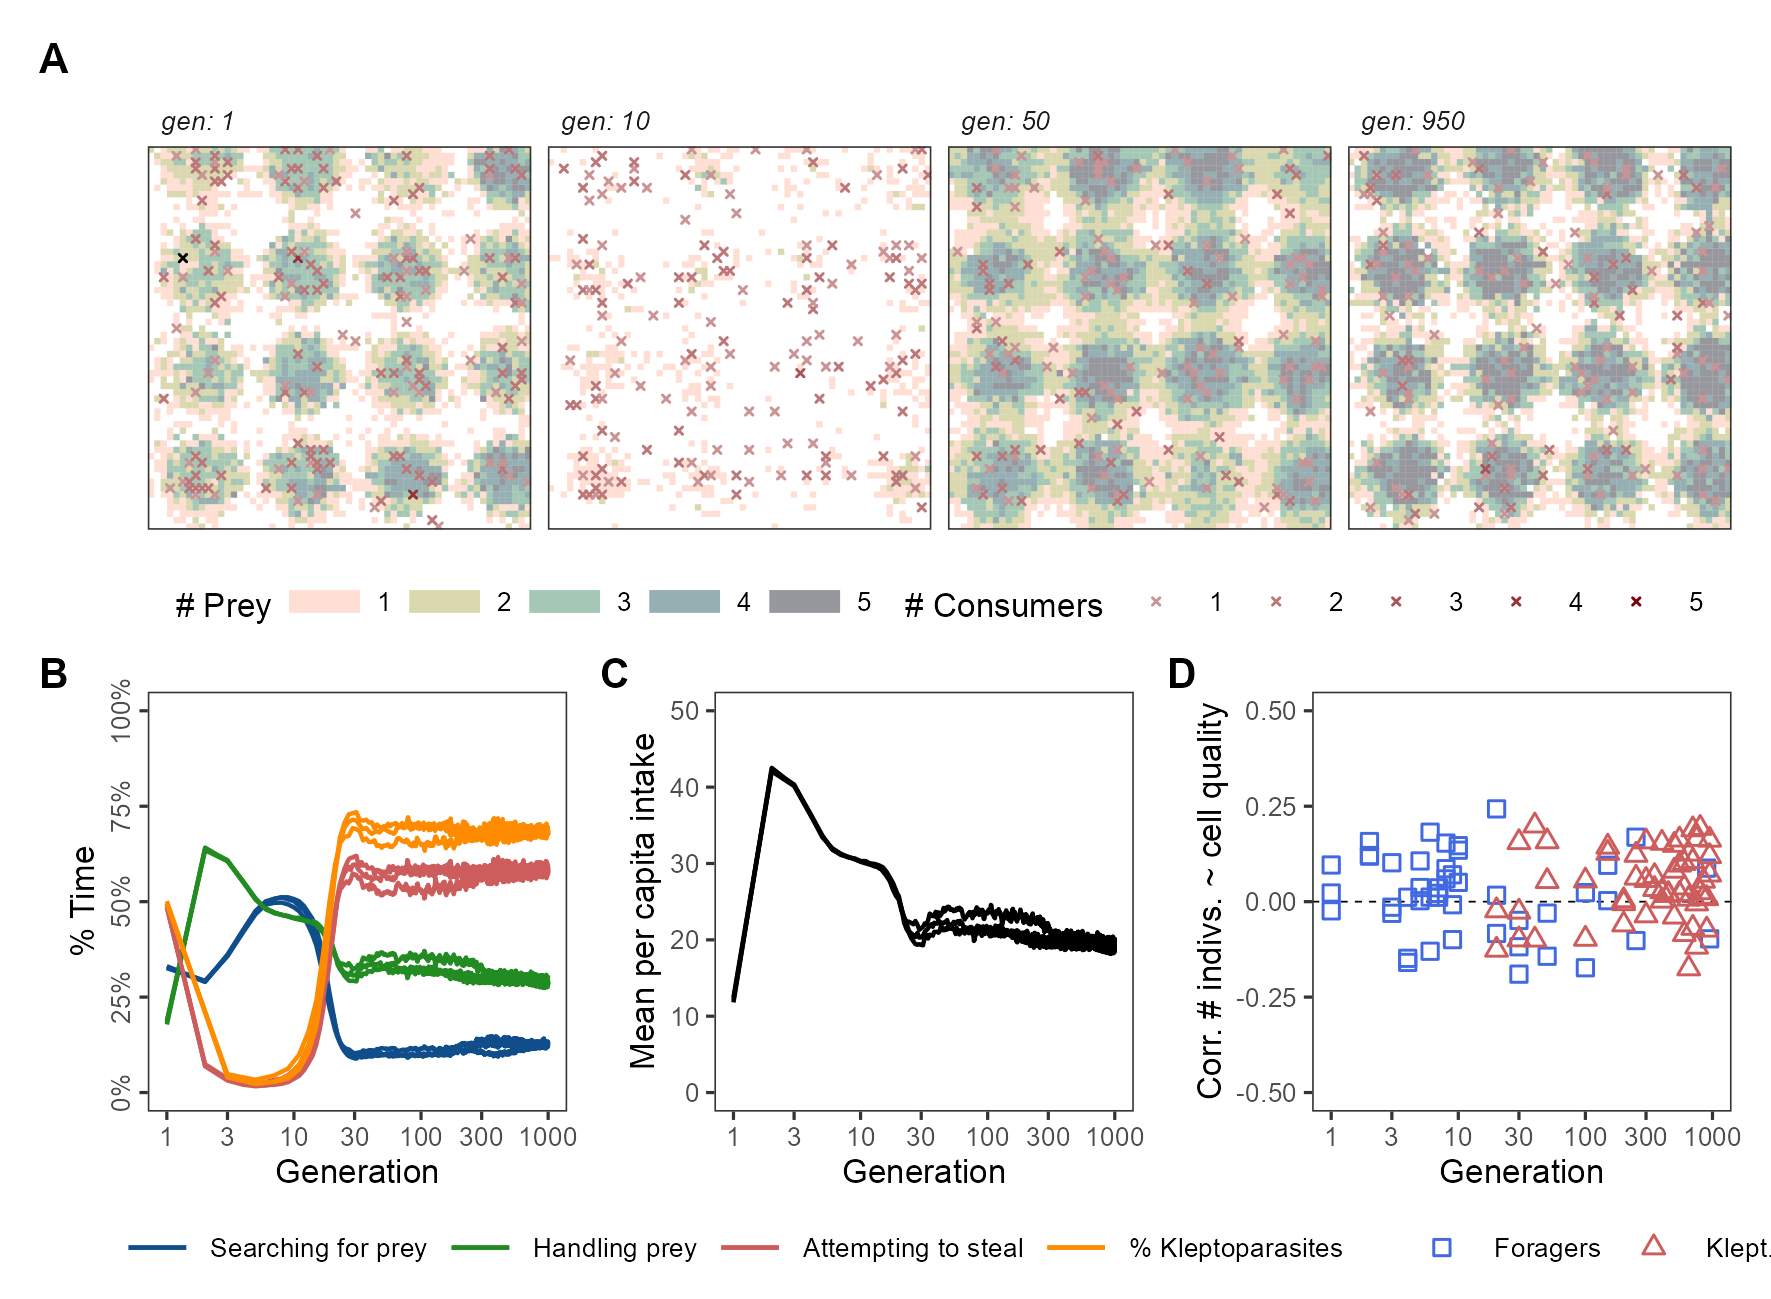
\includegraphics[width=0.9\textwidth]{figures/kleptomove/fig_02.png}
    \caption{
        \textbf{Eco-evolutionary implications of the coexistence of foragers and kleptoparasites following fixed competition strategies in scenario 2.}
        \textbf{(A)} Populations with both foragers and kleptoparasites drastically deplete the initially well-stocked resource landscape by generation 10; however, prey densities recover strongly by generation 50, even beyond the densities in generation 1.
        \textbf{(B)} A surprisingly stable equilibrium between the forager and kleptoparasite strategies is reached within 30 generations, with the relative frequency of kleptoparasites (orange line) first dropping to very low levels but later recovering to reach a high level ($\sim$ 70\%) in all three replicates.
        Consequently, at equilibrium, only about 10\% of individuals are foragers searching for prey, 50\% are kleptoparasites attempting to steal from handlers, and 40\% are handlers processing prey-items (either foragers or kleptoparasites). 
        \textbf{(C)} When kleptoparasites are rare, the population intake rate exhibits the same pattern as in scenario 1, dropping to a lower level with the emergence of kleptoparasites.
        Naturally, there is an increase in the proportion of time spent on stealing attempts (red line -- \textbf{B}), and a corresponding decrease in prey seeking (by searching foragers; blue line -- \textbf{B}), and handling (green line -- \textbf{C}).
        \textbf{(D)} Neither foragers nor kleptoparasites follow the input matching rule, and the correlation of their abundance with cell productivity $r$ is zero at equilibrium.
        Panel \textbf{A} shows a single replicate, while \textbf{B, C, D} and \textbf{D} show three replicates with log-scaled X-axes; all panels are for $r_{max}$ = 0.01.
    }
    \label{klepto_fig_02}
\end{figure}

\begin{figure}[t!]
    \centering
    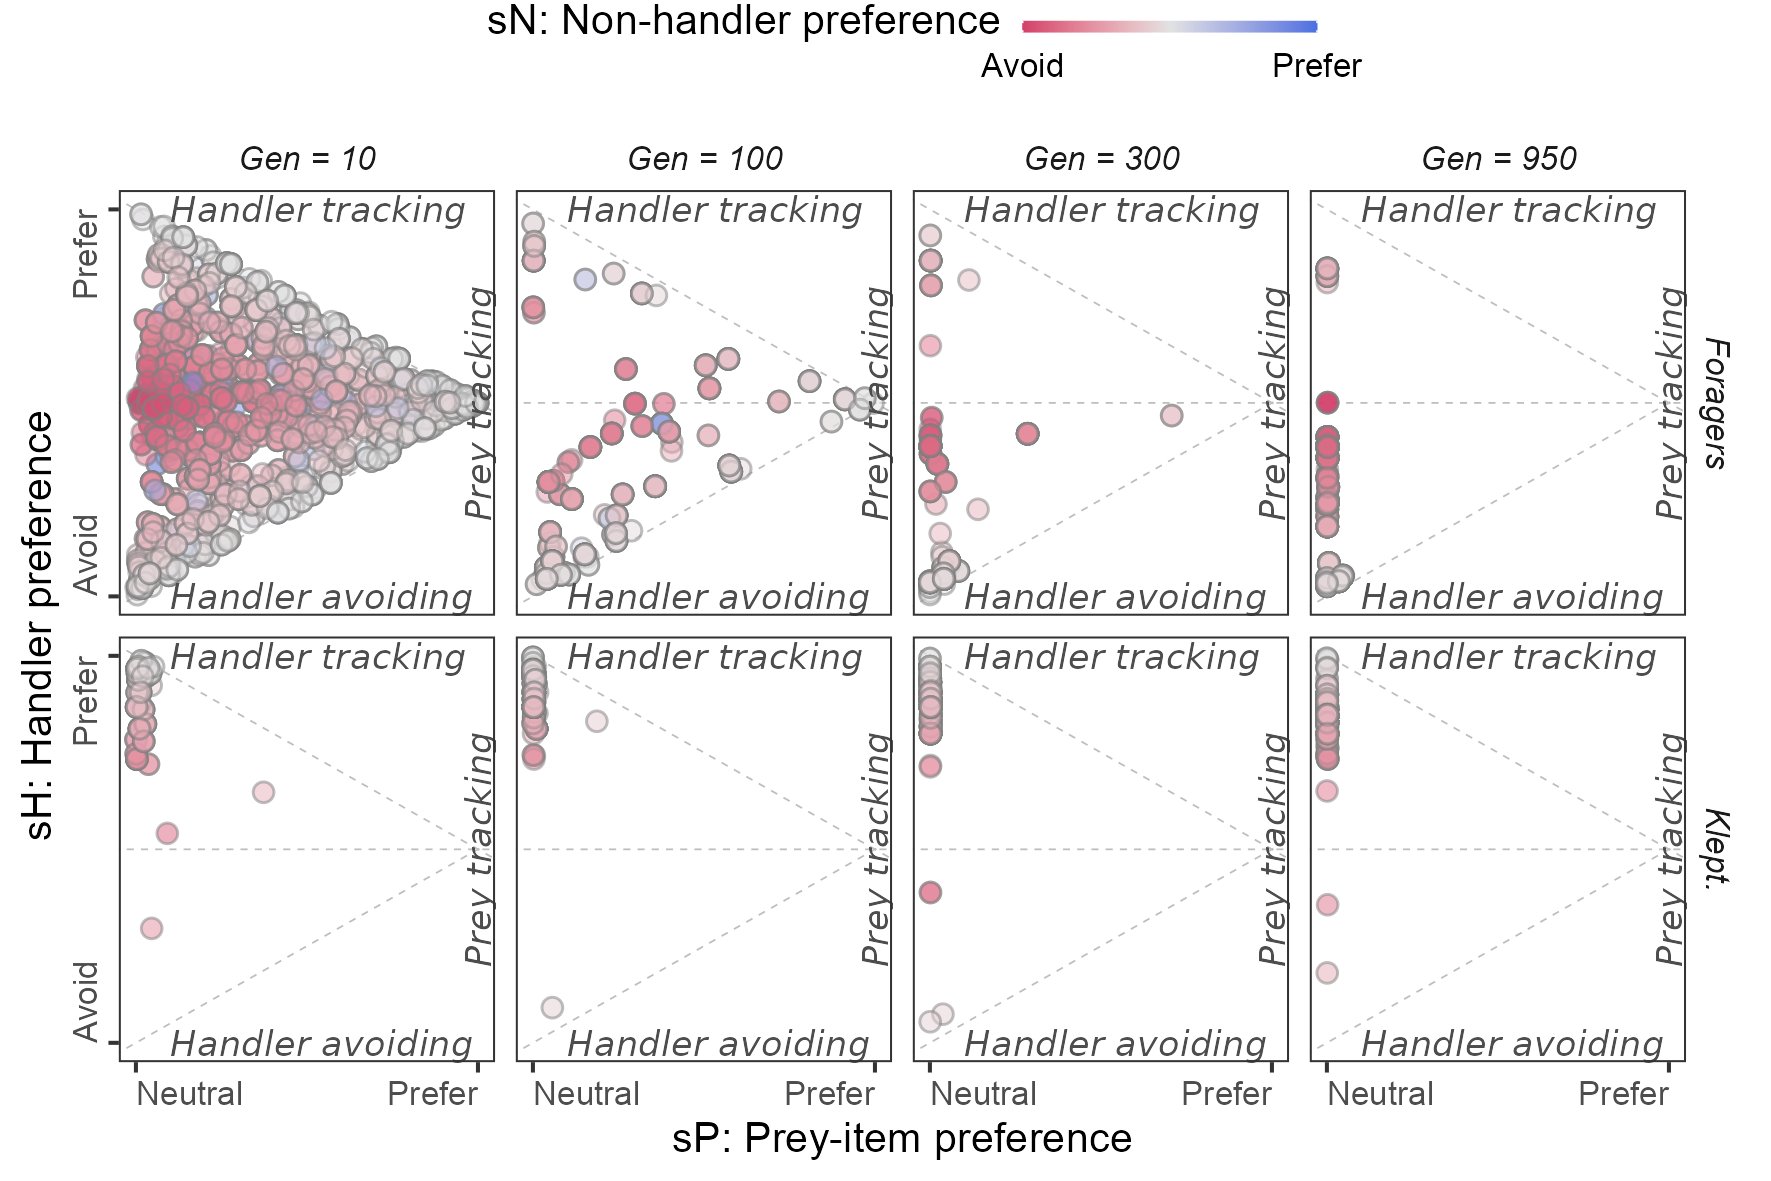
\includegraphics[width=0.9\textwidth]{figures/kleptomove/fig_03.png}
    \caption{
       \textbf{Rapid divergence of movement strategies between foragers and kleptoparasites in scenario 2.}
       In scenario 2, kleptoparasites rapidly diverge (within 10 generations) from foragers in their movement strategy, clustering around sH = 1.0: a handler-tracking strategy.
       This strategy is stably maintained throughout the simulation (G = 100, 300, 950).
       Foragers retain substantial diversity in movement strategies for many generations (see G = 100), but unlike scenario 1, tend to be repelled (relative sH < 0), as well as attracted to handlers (relative sH > 0).
       Over time, foragers adopt a strategy that helps them avoid all other individuals (G = 300, 950).
       A few individuals sporadically adopt a movement strategy associated with the opposite competition strategy; this is most likely due to mutations in the competition strategy, rather than a new movement morph within either foragers or kleptoparasites.
       At the evolutionary equilibrium then, social information (either sH or sN) is the strongest component of all individuals' movement strategies.
       All panels show 2,500 individuals (25\% of total) from the same simulation replicate ($r_{max}$ = 0.01), and earlier generations are ancestors of later generations.
    }
    \label{klepto_fig_03}
\end{figure}

\subsection*{Scenario 3: Condition-dependent Kleptoparasitism}

When individuals are allowed to choose their competition strategy (foraging or kleptoparasitism) based on local environmental cues, the distribution of prey-items is substantially different from the two previous scenarios (Fig.~\ref{klepto_fig_04}A).
Initially, individuals deplete the resource landscape of prey-items within ten generations.
By generation 50, the resource landscape recovers some of the spatial structure of early generations, but prey-item abundances do not match the recovery seen in scenario 2.
This is because unlike scenario 2, individuals search for prey more often and steal less (at or below 25\%; compare Figs.~\ref{klepto_fig_04}B and \ref{klepto_fig_02}B), preventing a full recovery of the resource landscape.
Consequently, mean per-capita intake stabilises (after an initial spike, as in scenarios 1 and 2) within ten generations to a level similar to scenario 1 (Fig.~\ref{klepto_fig_04}C).
While not as strong as predicted by IFD theory, the correlations between consumer abundance and cell productivity are weakly positive (Fig.~\ref{klepto_fig_04}D).

The weak input matching is likely because all individuals prefer to move up gradients of prey density, and towards handlers, which are more likely to be found on resource peaks (Fig.~\ref{klepto_fig_04}E; see also Supplementary Material Fig.~4, 7).
Using conditional foraging strategies, individuals are able to switch between resource types (prey and handlers) depending on which is more profitable \citep{emlen1966} (`opportunistic kleptoparasitism'; Fig.~\ref{klepto_fig_04}F; see Supplementary Material Fig. 6).
All individuals would choose to steal when handlers are present, even when prey items are more common.
Indeed, about 40\% of individuals would choose to steal even when prey are abundant and there are no handlers at all, showing the prevalence of a `fixed kleptoparasite' clade similar to scenario 2.
In a further parallel with scenario 2, about 70\% of individuals have an intrinsic bias towards kleptoparasitism, i.e., they would by default attempt to steal when there are no cues to inform their decision (Fig.~\ref{klepto_fig_04}F: $P$ = 0, $H$ = 0).

\begin{figure}[t!]
    \centering
    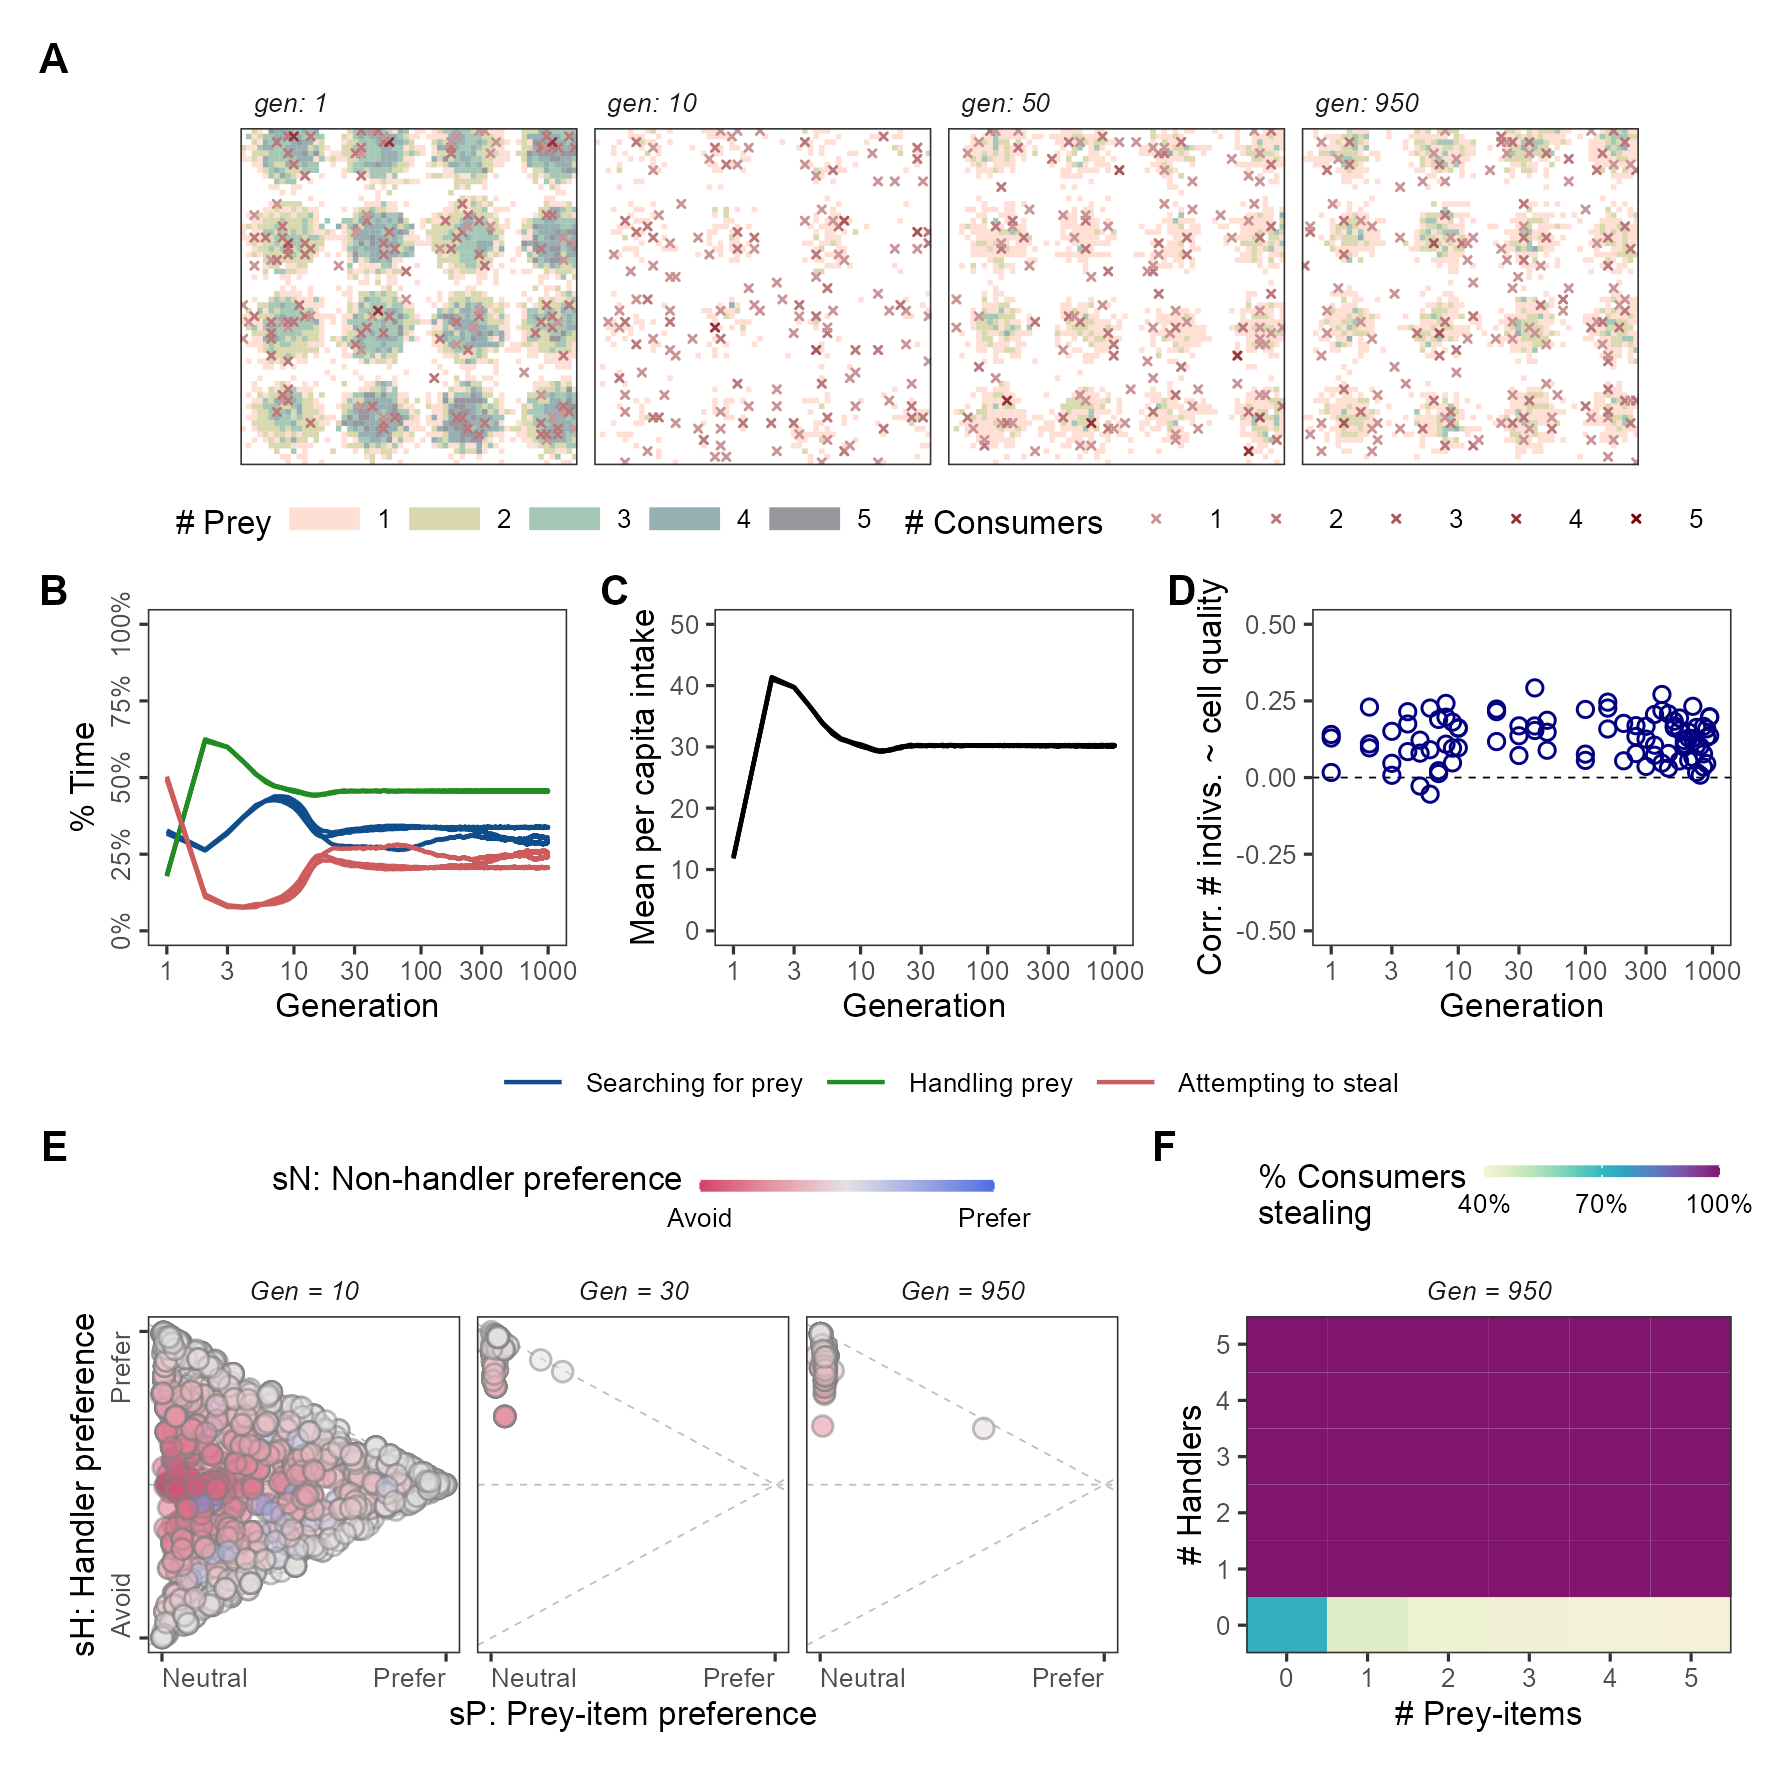
\includegraphics[width=0.9\textwidth]{figures/kleptomove/fig_04.png}
    \caption{
        \textbf{Eco-evolutionary implications of conditional foraging strategies in scenario 3.}
        \textbf{(A)} The initially well-stocked resource landscape is rapidly depleted within 10 generations, yet within 50 generations, prey abundances recover on many cells, though not to the extent of scenario 2.
        The local density of individuals on occupied cells is shown as coloured crosses. 
        \textbf{(B)} By generation 30, the proportion of time spent searching (blue line), handling (green line), and stealing prey (red line) reach an equilibrium that differs somewhat across replicates, but \textbf{(C)} the total intake of the population reaches the same equilibrium value in all three replicates.
        \textbf{(D)} The correlation between the local density of individuals on a cell, and its productivity $r$ is stronger than in scenario 2.
        \textbf{(E)} From an initially high diversity of movement strategies, there is a rapid convergence (within 30 generations) of all individuals to strongly prefer moving towards successful foragers, or handlers, nearly to the exclusion of all other movement cues.
        This handler-tracking strategy once established is maintained (Gen = 300, 950).
        \textbf{(F)} Population competition strategies are more varied. While most individuals will choose to forage as prey density increases, about 40\% of individuals attempt to steal even when prey is abundant and handlers are scarce.
        All individuals will steal when handlers are available.
        Panels \textbf{A, E} show a single replicate, while \textbf{B, C} and \textbf{D} show three replicates, \textbf{F} shows the mean across replicates; all panels are for $r_{max}$ = 0.01.
    }
    \label{klepto_fig_04}
\end{figure}

\subsection*{Movement Strategies on Depleted Landscapes}

Orienting movement towards resources \citep[][\textit{where to move}]{nathan2008a} can be a challenge in a system with low densities of discrete prey-items, because the local prey \textit{density} may provide very limited information about local \textit{productivity}.
In our model, prey-depletion leads parts of the resource landscape to become `clueless regions' \citep{perkins1992}, where foragers cannot make directed movements based on prey-item abundances alone, as all neighbouring item abundances are identical (see white areas in Fig.~\ref{klepto_fig_05}A; A1: scenario 1, A2: scenario 2, A3: scenario 3).
At the beginning of all three scenarios, about 75\% of landscape cells have a different number of prey-items from the cells around them; these are primarily cells with an intermediate $r$, which have more prey than peripheral cells of resource peaks, but fewer prey than the central cells.
This proportion rapidly declines to a much lower value within 10 generations in all three scenarios.

The `cluelessness' of the landscapes develops differently across scenarios on evolutionary timescales (Fig.~\ref{klepto_fig_05}B).
In scenario 1, the proportion of cells with a different number of items in the neighbourhood is initially very high (Fig.~\ref{klepto_fig_05}A1).
This proportion rapidly declines to $\sim$25\% within 10 generations, as foragers deplete most prey-items, making most of the landscape a clueless region.
In this context, foragers evolve to move towards handlers, with $>$ 75\% of individuals showing a preference for handlers within 100 generations (Fig.~\ref{klepto_fig_05}B1).
Forager preference for handlers may be explained as the sensing of a long-term cue of local productivity.
Since handlers are immobilised on the cell where they find a prey-item, handler density is an indirect indicator of cell $r$, and due to spatial autocorrelation, also of the $r$ of bordering cells.

Scenario 2 landscapes develop similarly to scenario 1 in early generations (Fig.~\ref{klepto_fig_05}A2).
However, within 50 generations, most cells bear items as extraction is reduced, with differences among cells according to their $r$ (see also Fig.~\ref{klepto_fig_02}A).
Thus $>$ 75\% of cells have a different number of items from neighbouring cells (Fig.~\ref{klepto_fig_05}A2 -- panel \textit{gen: 50}, 5B2).
Unlike scenario 1, the rapid increase in handler preference is driven by kleptoparasites becoming the majority strategy (see above).
Scenario 3 is similar to scenario 2, except that only about half of all cells have a different number of prey-items from neighbouring cells (Fig.~\ref{klepto_fig_05}A3, 5B3).
Here, the rapid evolution of a handler preference in movement decisions cannot be assigned a clear cause, since handlers are both a potential direct resource as well as indirect cues to the location of productive cells.

\begin{figure}[t!]
    \centering
    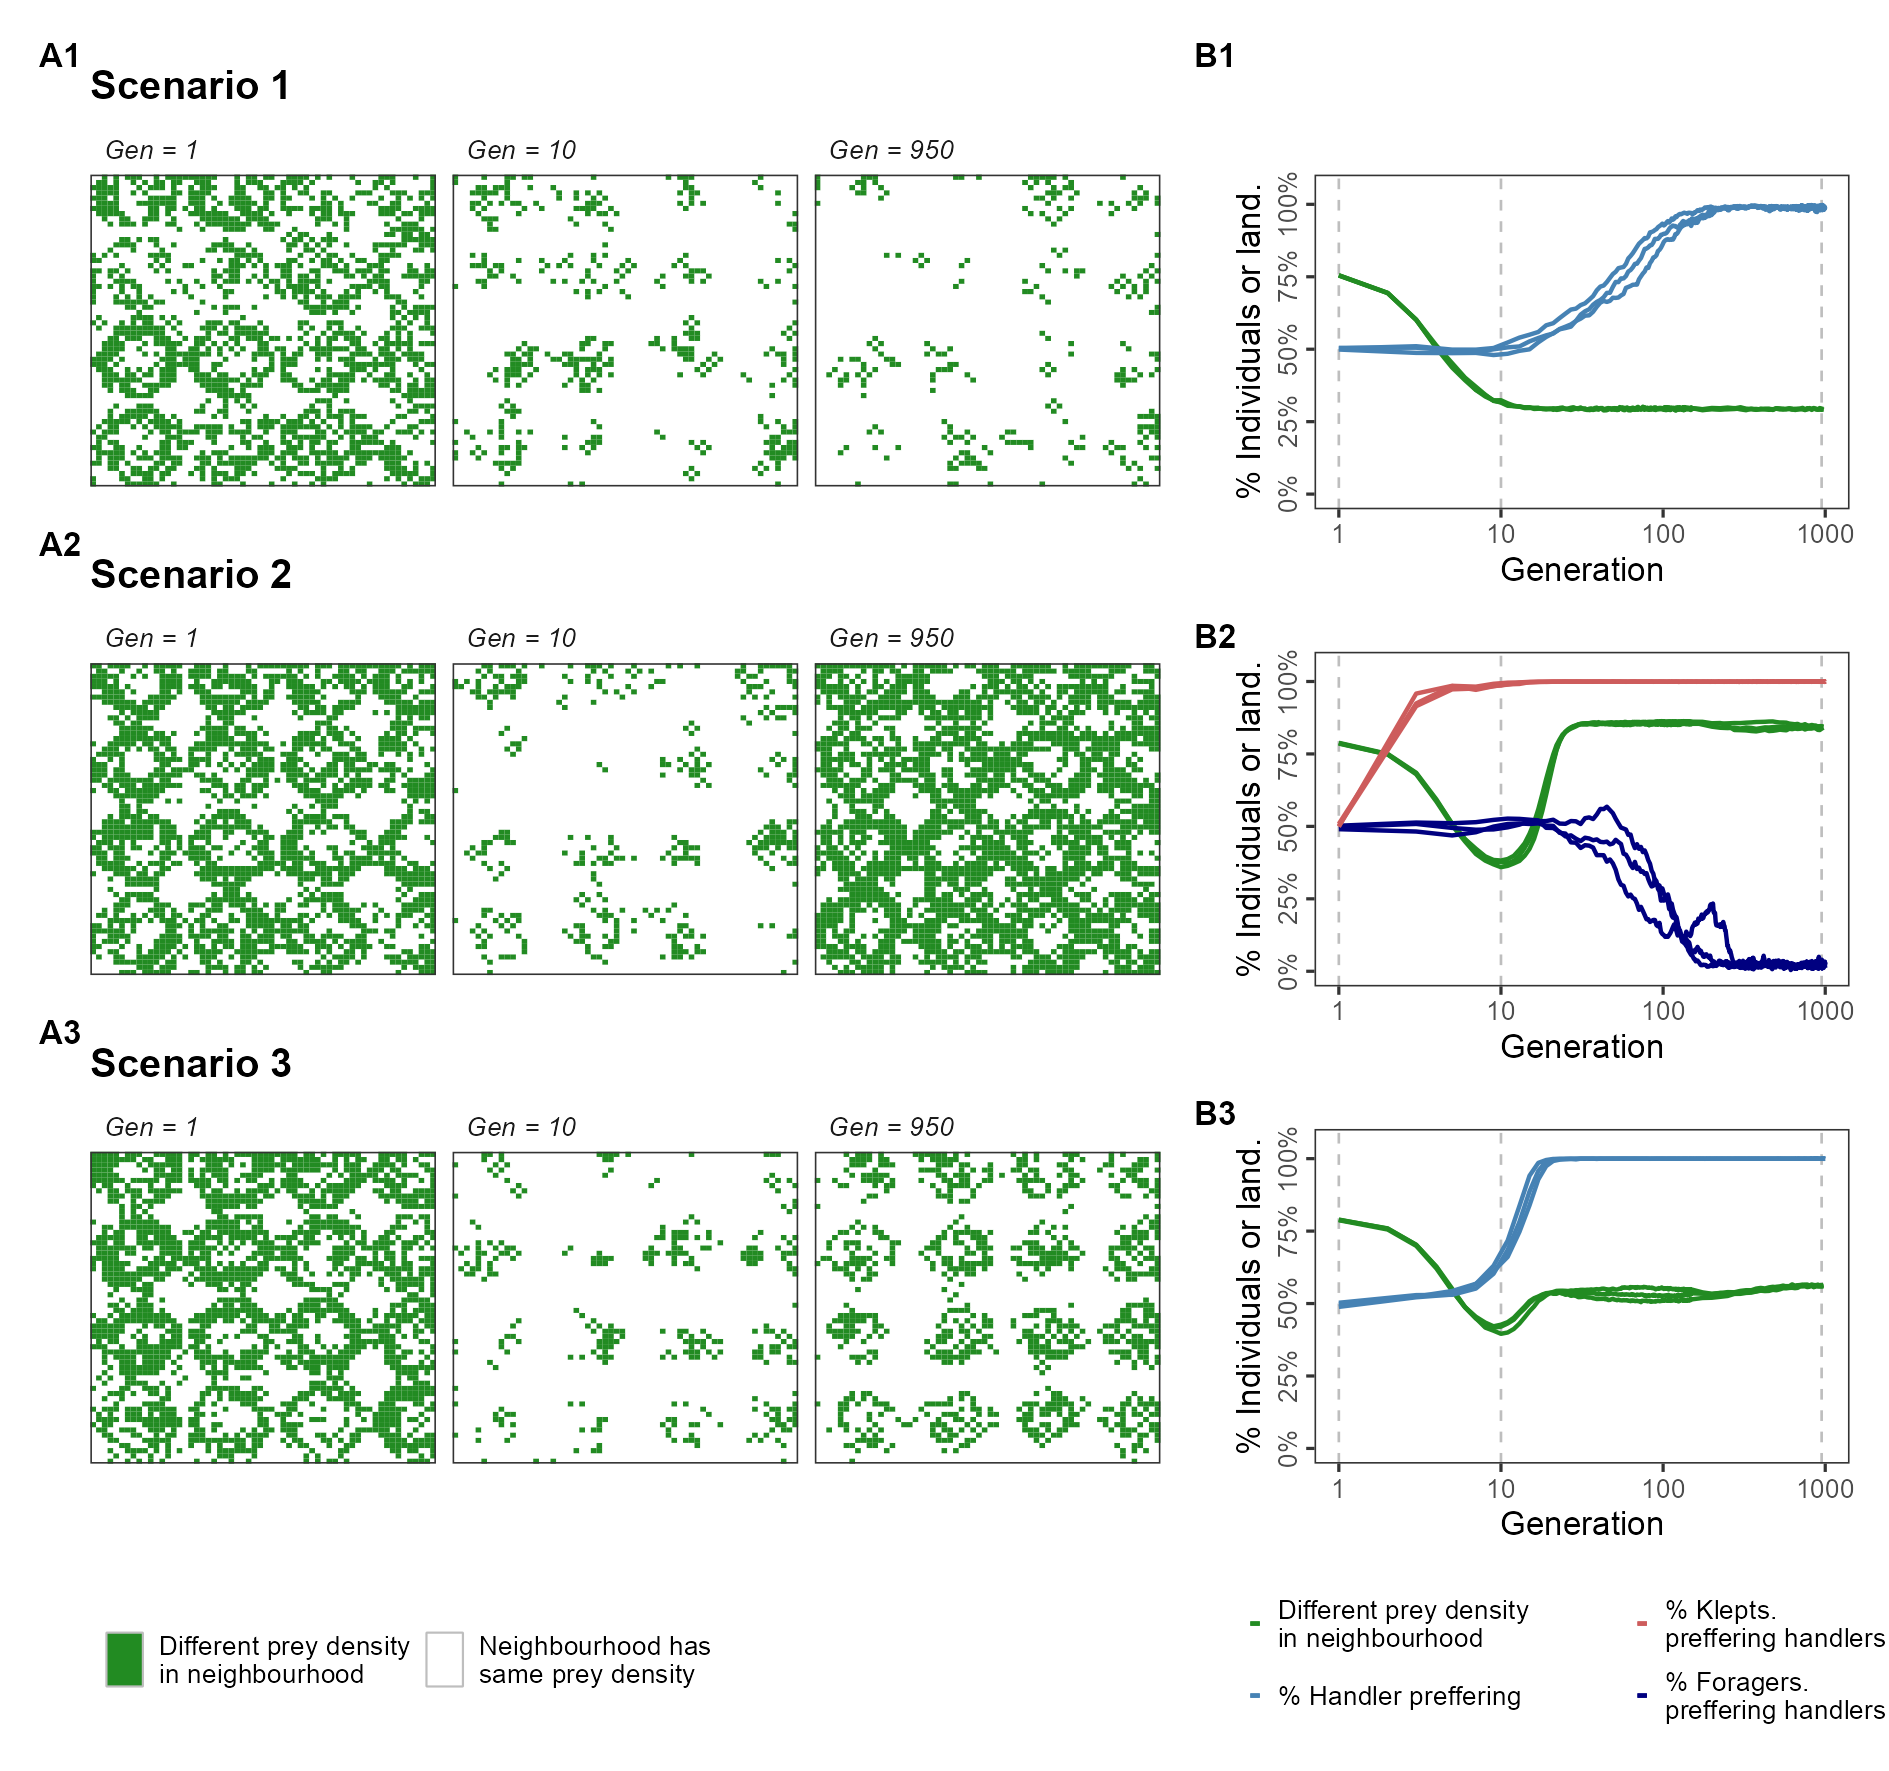
\includegraphics[width=0.9\textwidth]{figures/kleptomove/fig_05.png}
    \caption{
        \textbf{Uninformative prey densities and the evolution of social information as an alternative movement cue.}
        \textbf{(A1, A2, A3)} On cells coloured green, local prey densities are informative for movement, as the central and neighbouring cells have different prey densities.
        While differences in local prey densities provide informative cues for `adaptive' movement in early generations, this is much less true once the resource landscape is depleted of prey-items (depending on the scenario).
        \textbf{(B1, B2, B3)} The proportion of cells where differences in local prey densities provide informative movement cues (green line), and the proportion of individuals preferring to move towards handlers (blue line), whose presence may be used as an alternative cue for movement towards higher-productivity areas of the landscape.
        In \textbf{(B2)} representing scenario 2, this proportion is shown separately for foragers (blue line) and kleptoparasites (red line).
        While panels in \textbf{(A)} show a single representative replicate for $r_{max}$ = 0.01, panels in \textbf{(B)} show three replicates.
    }
    \label{klepto_fig_05}
\end{figure}

\subsection*{Effect of Landscape Productivity}

The prey-item regrowth rate that characterises the peaks of the resource landscape ($r_{max}$) is a measure of the productivity of the resource landscape overall. 
Having thus far focused on scenarios with $r_{max}$ = 0.01 (corresponding to a peak production of 4 food times per consumer lifetime), we find that, not unexpectedly, the value of $r_{max}$ has a marked effect on evolved population activity budgets, mean per capita intake, and even evolved strategies.
The frequency of foraging reduces with $r_{max}$ in scenarios 1 and 3; this is caused by more frequent acquisition of prey-items (as regrowth keeps pace with depletion), which results in a greater frequency of handling rather than foraging.

In scenario 2 however, the frequency of handling is relatively unaffected by increasing $r_{max}$ (Fig.~\ref{klepto_fig_06}A).
The difference between scenarios 2 and 3 has to do with the change in the frequency of kleptoparasitism (Fig.~\ref{klepto_fig_06}B).
In scenario 2, kleptoparasitism forms $>$ 75\% of all activities at low $r_{max}$, and is much more common than in scenario 3 populations at the same regrowth rate.
However, at relatively high $r_{max}$ (0.03), the fixed kleptoparasitic strategy goes extinct.
This is because at high $r_{max}$, forager-prey encounters are more common than kleptoparasite-handler encounters, in both early ($<$ 10) and later generations ($>$ 50).
Consequently, kleptoparasites have relatively much lower fitness than foragers, and do not proliferate.
Thus at high $r_{max}$, a scenario 2 population is nearly identical to a scenario 1 population; while some kleptoparasites may be seen in later generations, these occur most likely due to ephemeral mutations in the forager strategy.

In scenario 3, kleptoparasitism persists at low frequencies even at the highest regrowth rates (Fig.~\ref{klepto_fig_06}B); thus some foragers lose time in extracting items which are then stolen from them.
Consequently, while populations in all three scenarios achieve very similar mean per-capita intakes at low $r_{max}$, at intermediate regrowth rates (0.01, 0.02), conditionally kleptoparasitic populations achieve a higher mean per-capita intake than populations using fixed strategies.
Only at high $r_{max}$, when fixed strategy populations effectively convert to purely forager populations, do they achieve a higher intake than conditional strategy populations (Fig.~\ref{klepto_fig_06}C).

\begin{figure}[t!]
    \centering
    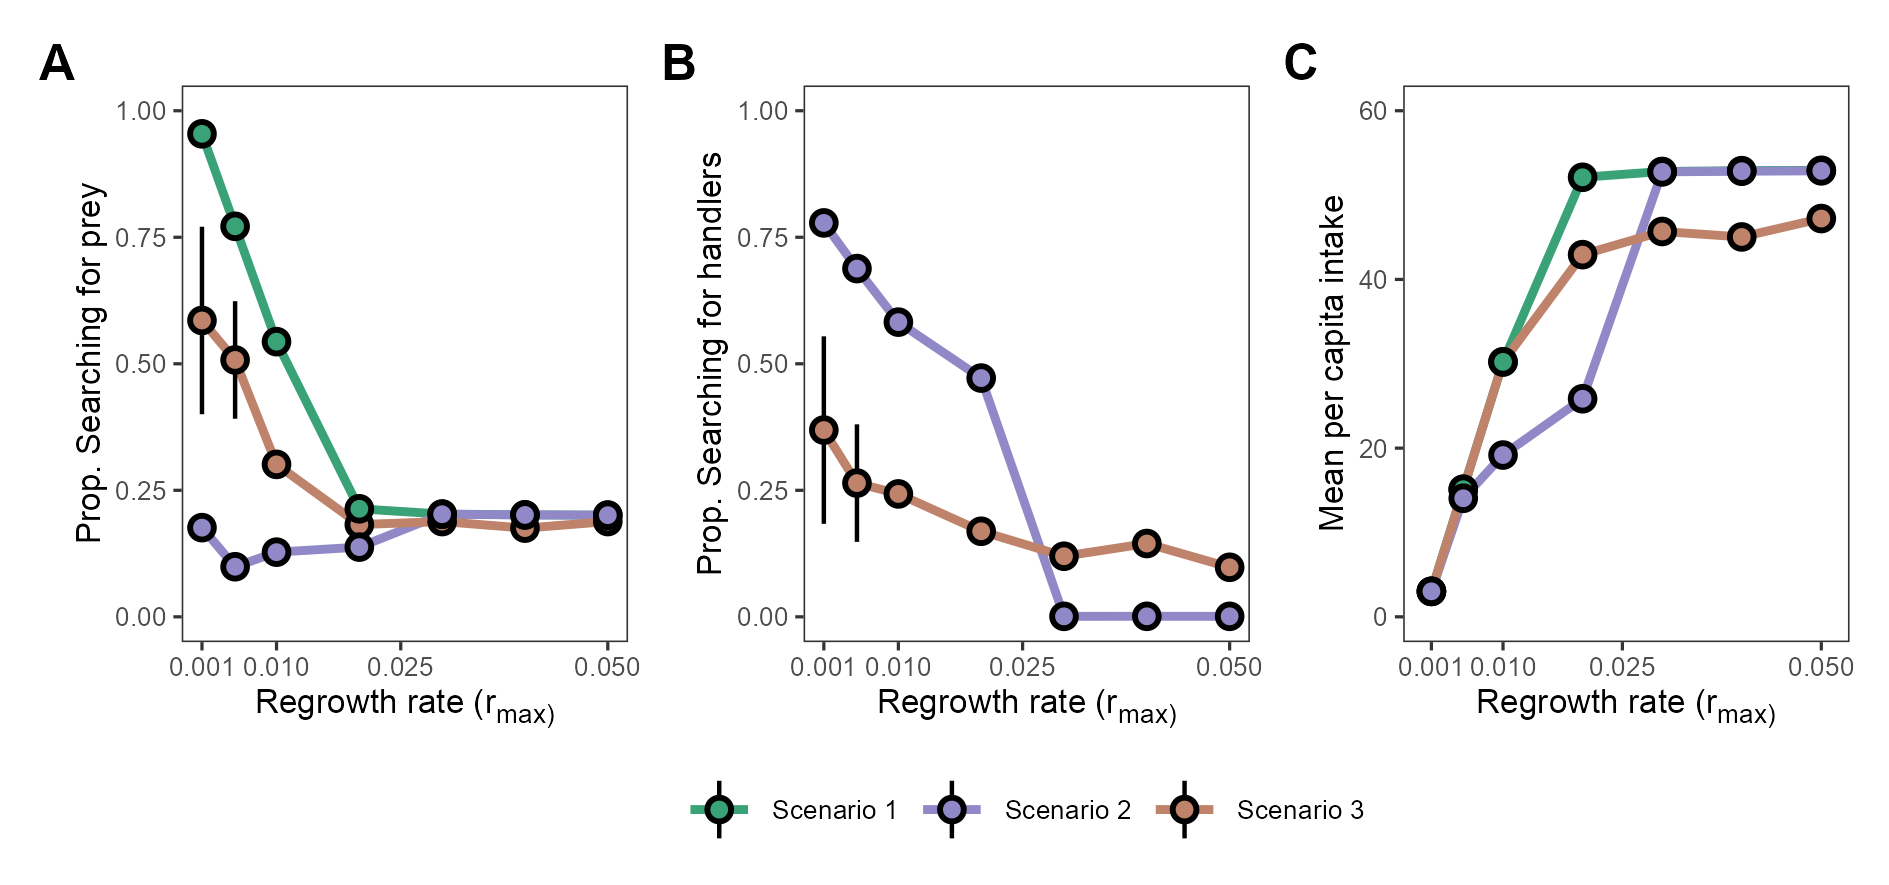
\includegraphics[width=\textwidth]{figures/kleptomove/fig_06.png}
    \caption{
        \textbf{Landscape productivity strongly affects scenario outcomes.}
        \textbf{(A)} The proportion of time spent searching for food decreases with increasing $r_{max}$ in scenarios 1 and 3 but remains relatively stable within scenarios. 
        This is partly due to a higher proportion of time spent handling at higher prey densities. 
        \textbf{(B)} The proportion of time spent searching for handlers (in order to steal prey from them) also decreases with increasing $r_{max}$. 
        In scenario 2, kleptoparasites go extinct for $r_{max}$ values above 0.025. 
        \textbf{(C)} At low productivity, the average intake is similar in all three scenarios. 
        For higher $r_{max}$ values the average intake rate is lowest in scenario 2, until $r_{max}$ is larger than 0.025 and kleptoparasites go extinct (leading to the same kind of population as in scenario 1). 
        At high $r_{max}$, the average intake rate in populations with conditional kleptoparasites (scenario 3) is substantially lower than in populations without kleptoparasitism.
        All panels show conditions at G = 1,000; error ranges where present show standard deviation around values; some error ranges are too small to be visible.
    }
    \label{klepto_fig_06}
\end{figure}

\section*{Discussion}

Our spatially-explicit individual-based model implements the ecology and evolution of movement and foraging decisions, as well as resource dynamics, in biologically plausible ways, and offers a new perspective on the distribution of animals in relation to their resources under different scenarios of competition.
%%
First, individuals moving with a limited perception range and competing only by exploitation, evolve movement strategies for both direct and indirect resource cues (prey-items and handlers, respectively).
Regardless, on a resource landscape with discrete prey-items, large areas may become devoid of any movement cues, leading to a mismatch between individual distribution, prey-item distribution, and landscape productivity.
%%
Second, interference competition in the form of kleptoparasitism rapidly establishes itself on landscapes where stealing is more time-efficient than searching for prey, even when such interference is a fixed strategy and kleptoparasites cannot forage for prey.
This rapid increase in kleptoparasitism as a strategy is accompanied by the divergent evolution of movement strategies that favour moving towards handlers, which are the primary resource of the kleptoparasites.
In this sense, obligate kleptoparasites may be thought of as forming a higher trophic level, with handlers as their prey.
%%
Third, when foraging strategy is allowed to be conditional on local cues, \textit{(1)} the population's mean per capita intake is significantly higher than that of a population with fixed strategies, and \textit{(2)} unlike fixed strategy populations, kleptoparasitism as a strategy does not go extinct on high-productivity landscapes.
%%
However, across scenarios, individuals are broadly unable to match the productivity of the resource landscape, contrary to the predictions of IFD based models, which predict input matching for some \citep{parker1986,holmgren1995,hamilton2002}, or all of the competitive types \citep{korona1989}.

\subsection*{Comparison with Existing Models}

Existing models of competition and movement impose fixed movement rules on individuals to mimic either ideal or non-ideal individuals \citep{vickery1991,cressman2006,amano2006b,beauchamp2008,stillman2010,white2018}.
When individual competitive strategies are included in models, they represent differences in competitive ability \citep[e.g.][]{parker1986,holmgren1995,hamilton2002}, or a probabilistic switch between producing and scrounging \citep{beauchamp2008}.
In contrast, our model allows individuals' movement (and competition) decisions to be adaptive responses to local environmental cues.
Similar to \cite{getz2015,getz2016} and \cite{white2018}, our individuals choose from among the available movement options after weighing the local environmental cues, similar to step selection functions \citep{fortin2005, avgar2016, white2018}.
Local environmental cues are constantly changing, as we model discrete, depletable prey-items, contrasting with many IFD models \citep[][]{tregenza1995,amano2006b}.
This allows for a more plausible, fine-scale consideration of exploitation competition, which is often neglected, and allows the cues sensed by individuals to strongly structure the distribution of competitors (see below).

Adaptive responses must have an explicit evolutionary context, and consider multiple generations of the population.
We follow \cite{beauchamp2008} and \cite{getz2015} in allowing the cue preferences that decide movement, and variation therein, to be the outcomes of natural selection.
However, instead of using `evolutionary algorithms' \citep{beauchamp2008,getz2015,getz2016} to `optimise' individual movement rules, we consider a more plausible evolutionary process: \textit{(1)} Instead of allowing the fittest 50\% of the population to replicate, the number of offspring are proportional to individual fitness.
\textit{(2)} The cue preferences are subject to mutations independently, rather than subjecting all preferences of an individual to simultaneous mutation.
\textit{(3)} Finally, we avoided `simulated annealing', which adapts the mutation rate or the mutational step sizes to the rate of evolutionary change.
Instead we drew mutation sizes from a Cauchy distribution, so that most mutations are very small, but large-effect mutations do rarely occur throughout the simulation.
Similarly, rather than determining competition strategy probabilistically or ideally \citep{vickery1991,beauchamp2008,tania2012}, our individuals' competition decisions are also shaped by selection (in scenarios 2 and 3).

\subsection*{Evolution of Movement Strategies Using Social Information}

In scenario 1, depletion of discrete prey can leave many areas empty of prey-items: in such areas, movement informed by a resource gradient is impossible, and individuals may move randomly \citep[][]{perkins1992}.
This lack of direct resource cues for locally optimal movement might be among the mechanisms by which unsuitable `matrix' habitats modify animal movement on heterogeneous landscapes \citep{kuefler2010}.
When individuals do not sense resource gradients, the presence of more successful conspecifics may indicate a suitable foraging spot \citep[local enhancement;][]{giraldeau1999,beauchamp2008,cortes-avizanda2014}.
The presence of unsuccessful individuals, meanwhile, may signal potential costs from exploitation or interference competition.
This selects for movement strategies incorporating the presence and condition of competitors into individual movement decisions, or \textit{social movement strategies} \citep[see e.g.][]{guttal2010}.
Consequently, consumer aggregation --- often explained by invoking external costs such as predation \citep{krause2002,folmer2012} --- could also be the outcome of movement strategies that have evolved to trade competition costs for valuable social information on the underlying spatial structure (here, $r$) of uninformative landscapes \citep[][]{folmer2010,cortes-avizanda2014}.

\subsection*{Individual Variation in Movement Strategies}

Our movement strategies, comprising preferences for local ecological cues, may lead individuals to move in ways that are potentially unique to each individual.
These strategies may not maximise their intake over short timescales (a few timesteps), but their coexistance implies equivalent fitness overall.
This makes them consistent with prevalent ideas about consistent individual differences in behaviour, or `animal personalities' \citep{wolf2012,laskowski2013,spiegel2017,shaw2020}.
In scenario 1, the persistence of multiple movement strategies across generations indicates that they have equivalent fitness \citep[see][]{getz2015}, and that there are multiple ways to navigate a heterogeneous environment \citep{wolf2010,shaw2020}.
Such differences may help reduce competition as individuals make subtly different movement decisions when presented with the same cues \citep[][]{wolf2012,laskowski2013}.
Interestingly, scenario 3 has the least individual variation in movement rules, presumably because plasticity in competition strategy reduces the need for such diversification \citep{pfennig2010}.

Scenario 2 cautions that \textit{(1)} Individual variation may only be evident when accounting for the main driver of movement decisions ($s_H$ or $s_N$; {see Supplementary Material Fig. 8 for scenario 3 as well).
\textit{(2)} Spatial context determines whether individual differences in movement strategy lead to functional variation in movement outcomes.
Subtle variation in relative prey density preferences ($s_P$) could be revealed if individuals were measured in isolation, and could lead to differences in movement paths (given a continuous gradient in prey cues).
However, in natural settings with substantial collective behaviour, different social movement strategies (correlated with foraging competition strategy) would be the primary driver of movement.
Overall, then, \textit{(a)} measuring movement behaviour in settings that correspond to animals' evolutionary context, and \textit{(b)} accounting for movement-competition strategy correlations, are both key when studying how individual differences translate to functional consequences.

\subsection*{Competition Strategies and the Ideal Free Distribution}

IFD models predict that individual movement should result in consumer distributions tracking the profitability of resource patches \citep{fretwell1970,parker1978}, with dominant competitive types (including kleptoparasites) monopolising the best patches \citep[][]{parker1986,holmgren1995,hamilton2002}, though \citet{korona1989} predicts otherwise.
In scenarios 2 and 3, kleptoparasitic individuals unsurprisingly and rapidly evolve to track handlers (a direct resource), while avoiding non-handlers (potential competitors).
However, these evolved rules do not lead kleptoparasites to occupy the best cells as predicted by \citealp{parker1986}, \citealp{holmgren1995}, and \citealp{hamilton2002}.
Across our scenarios (including scenario 1), local population density is only weakly correlated with cell productivity, and is not stronger than if individuals were moving randomly (see Supplementary Material Fig. 1).
In scenario 2, this departure from predictions is driven by the contrasting movement rules of foragers, which evolve to \textit{avoid} handlers as well as non-handlers, both of which might be kleptoparasites \citep[cryptic interference; seen in interference-sensitive shorebirds][]{bijleveld2012}.
Thus, foragers likely avoid resource peaks, which are more likely to have handlers \citep[due to the higher probability of forager-prey encounters][]{parker1986,holmgren1995,hamilton2002}.
Fixed kleptoparasites cannot extract prey themselves, and must move off resource peaks to track and rob handlers \citep[similar to][]{parker1986}, breaking the link between individual density and productivity.
This shows the pitfalls of simplistically linking current ecological conditions with population distributions without considering competitive strategies or evolutionary history.

\subsection*{Constraints on Competition Strategies}

Foraging strategies involving specialisation on a resource type are expected to be constrained by the availability of that resource. 
Thus kleptoparasitism, seen as a prey-choice problem, should be constrained by the density of targets \citep{ens1990}.
In scenarios 2 and 3, more kleptoparasitism should be expected with increasing $r_{max}$, as prey and consequently, handlers, are expected to be more abundant.
Instead, kleptoparasitism declines with increasing $r_{max}$, in line with \cite{emlen1966}, who predicted that the commoner food type (prey) rather than the more efficiently exploited one (handlers) should be preferred.
This prey choice problem, playing out at evolutionary scales, leads kleptoparasites in scenario 2 to go extinct when prey are very common at high $r_{max}$.
At stable population densities, the persistence of fixed kleptoparasitism depends on their intake \textit{relative to foragers}.
Modelling discrete prey-items and individuals in a spatial context, then, leads to the finding that obligate kleptoparasitism is only a viable strategy when forager-prey encounters are less common than kleptoparasite-handler encounters.
Reducing the relative profitability of kleptoparasitism in other ways --- such as imposing a cost on kleptoparasitic attacks for the initiator, or reducing the probability of success (currently, 1.0) --- would also lead to a reduced incidence of kleptoparasitism, and eventual extinction even on less productive landscapes.
In scenario 3, about 40\% of individuals choose to attempt to steal even when prey are available and handlers are not.
This suggests a more realistic proportion of consistently kleptoparasitic individuals among populations with flexible foraging strategies.
Many seabirds, which forage for prey when they are super-abundant, but also readily harass other birds for prey, are a good example \citep{brockmann1979}.
Finally, comparing across regrowth rates shows why possibly cryptic behavioral complexity should be considered in predictions of the long-term effect of environmental change on populations.
While both scenario 1 and 2 populations appear identical at high $r_{max}$, even a small decrease in environmental productivity could lead to an abrupt drop in per-capita intake --- and potentially, strongly reduced growth or survival --- for fixed strategy populations due to unexpected, emergent kleptoparasitism.

% \subsection*{Comparison with Conceptual Models}

% Classical models of animal movement and foraging largely consider homogeneous populations and environmental conditions, and movements that are made either optimally or at random.
% While these models provide powerful insights, 
% % they also have important drawbacks: individual variation, local environmental conditions, and the mechanisms of movement and decision-making cannot be adequately addressed. 
% % This is the strength of 
% individual-based models such as ours have the advantage that they can accommodate individual variation, local environmental conditions, and the mechanisms of movement and decision-making.
% % : the individual-level perspective can accommodate local circumstances, mechanisms and state variables in considerable depth and detail. 
% Individual-based modeling has the obvious drawback that numerous specific assumptions have to be made, which might not all be founded on empirical evidence, and might seem to limit the generality of the conclusions. 
% Nevertheless, as long as these models are not mistaken for attempts at faithful representations of real systems, their exploration provides valuable perspectives on the conceptual models that have dominated theory in the past. 
% After all, traditional models also include numerous assumptions (the spatio-temporal structure, the timing of events, the distribution and inheritance of traits) that are usually not stated and therefore less visible.
% For the future, we envisage pluralistic approaches, where both types of model are applied to the same research question. 
% Only comparing the outcomes of diverse models will reveal which conclusions and insights are robust, and which reflect peculiarities of the model structure.
% Only such model comparison can tell us whether and when simple models produce general insights, where simple models fail, and when mechanisms can explain initially counterintuitive observations, such as the attraction to competitors that we observed in our study.

\subsection*{Individual-Based Models in Animal Movement Ecology}

Linking individual-based models with empirical data is difficult, and is still rarely used \citep[see works tailored to management:][]{stillman2010,diaz2021}.
Animal tracking technology is only on the cusp of allowing us to track entire populations (though small ones), and classifying their behaviour at the fine temporal scales of animal decision-making \cite[Nathan et al. in press. \textit{Science}; see e.g.][]{lieber2021, sankey2021}.
Classifying dyadic and collective behaviour from animal tracking is especially challenging \citep{sankey2021,vissat2021}; this makes the detection of rapid competitive interactions in large populations unlikely.
Instead, experimental approaches may reveal movement strategies that reduce competitive interactions \citep{vahl2005,vahl2005a,rutten2010, bijleveld2012}.
However, consistent behaviour in cue-poor captive environments does not always translate to consistency in natural settings with abundant resource cues \citep{carter2013}.

Animal movement ecology takes an explicitly individual-based approach, centred around individual decisions \citep{nathan2008a}.
This makes individual-based models a good choice when seeking general insights into the evolutionary ecology of animal movement strategies \citep[see e.g.][]{getz2015}, whose ultimate causes are otherwise difficult to study empirically.
Modelling mechanistic movement decisions has substantial consequences for ecological outcomes \citep[e.g.][]{mueller2011,white2018,scherer2020}, yet few individual-based models in animal movement are mechanistic \citep[see review in:][]{deangelis2019}, and even fewer models include evolutionary dynamics \citep[but see][]{getz2015,getz2016,netz2021a}. 
Yet explicitly modelling both ecological interactions and evolutionary dynamics, as we do here, can reveal surprising outcomes ranging from innovative predator-prey strategies \citep{netz2021a} to sympatric speciation \citep{getz2016}.

The use of resource- and step-selection functions in mechanistic modelling \citep[see][]{white2018} gives empirical movement ecologists a familiar starting point in individual-based modelling.
Simulating an animal's potential space-use, conditional on environmental data (similar to our cues), and using selection coefficients estimated from tracking data (our cue preferences), is already accepted in movement ecology, and follows our grid-based approach \citep{avgar2016,signer2019,avgar2020,fieberg2021}.
It is relatively easy to implement movement decisions in continuous space, by sampling cues at discrete locations and \textit{(1)} choosing among them, or \textit{(2)} translating these cues into a movement distance and turning angle.
The second approach would require more complex functions with more coefficients (preferences), such as neural networks \citep{mueller2011}, and this could make it difficult to interpret the evolved movement strategies.
Models could implement survival and reproduction (the key ingredients of natural selection), as well as other demographic processes, and reproduction and inheritance can be incorporated in a more realistic manner.

We call for a substantial increase in mechanistic, evolutionary, individual-based modelling in animal movement ecology.
Adding realistic ecological and evolutionary dynamics on top of current empirical work is key to transforming movement ecology into a more applied, predictive discipline.
For example, by allowing habitat selection coefficients from animal-tracking studies to undergo even short-term selection on projected landscapes from climate modelling, such models could help explore population changes in movement strategies.
This approach would require very accurate estimation of the fitness outcomes of movement --- no easy task.
Consequently, individual-based models are not (yet) intended to be `fit' to empirical movement data.
Rather, they can provide valuable perspective on existing population-level models, and could be used to define the envelope of possibilities for how movement strategies could evolve in dynamic environments.

% \section*{Acknowledgments}

% We thank Hanno Hildenbrandt for contributing extensively to the coding of the simulation model \textit{Kleptomove};
% Matteo Pederboni for contributing to the model's development; 
% and members of the Modelling Adaptive Response Mechanisms Group, and of the Theoretical Biology department at the University of Groningen for helpful discussions on the manuscript.
% F.J.W. and C.F.G.N. acknowledge funding from the European Research Council (ERC Advanced Grant No. 789240).
% P.R.G was supported by an Adaptive Life Programme grant made possible by the Groningen Institute for Evolutionary Life Sciences (GELIFES).
% Finally, we thank two anonymous reviewers for helpful suggestions that improved the manuscript.

\newrefcontext[sorting=nyt]
\section*{Literature Cited}
\printbibliography[title={Literature~Cited},heading=none]
\end{refsection}